\section{Module 12. Oblique imaging}

\indent After clicking to run module 12 a new window is opened.

\begin{figure}[H]
\centering{}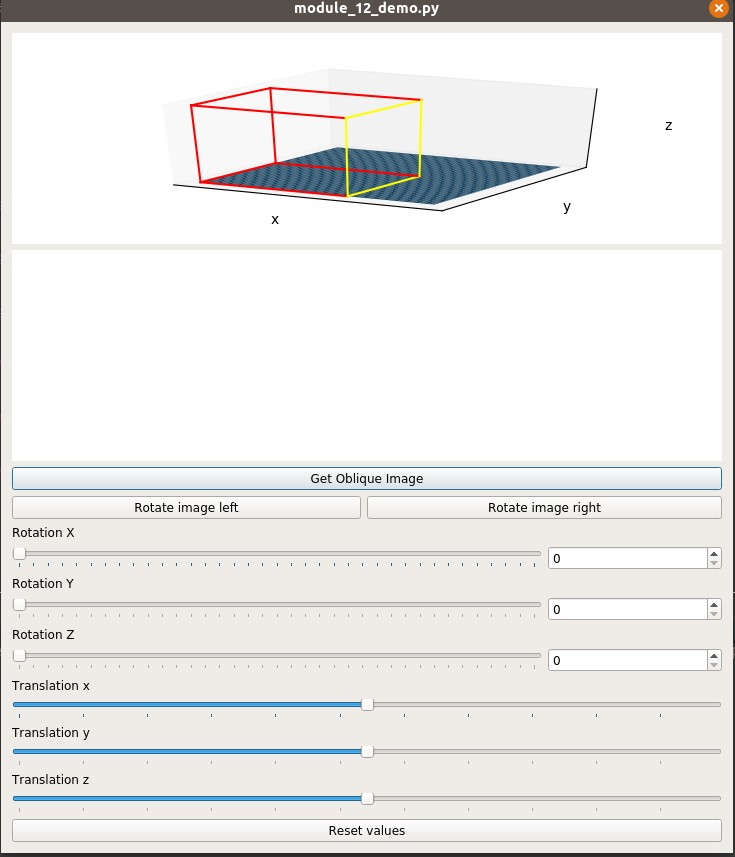
\includegraphics[scale=0.6]{figures/module_12/mod12window}\caption{Module 12 window\label{fig:figure/module_12/Preprocessing}}
\end{figure}

\indent In this window there are 2 plotting space 4 buttons : 'Get Oblique Image', 'Rotate image left','Rotate image right and 'Reset values'. There are also 6 sliders: 'Rotation X', 'Rotation Y', 'Rotation Z', 'Translation X', 'Translation Y', 'Translation Z' and 3 spinboxes responsible for 'Rotation X', 'Rotation Y', and 'Rotation Z'.
\newline\indent As can be seen on previous figure only grid and shape of the data in form of red and yellow lines (yellow lines mean the front of the data) is displayed and not the actual data itself. It is because displaying the data in matplotlib and updating the figure that displays it with the grid every time someone uses a slider or write a different value in a box might result in a really slow performance.
\newline\indent The view of this plot is default from the start of the module and can be changed manually at any moment. In order to change it user needs to press left button on the figure and slide in any direction.

\begin{figure}[H]
\centering{}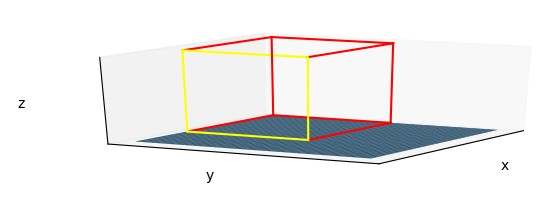
\includegraphics[scale=0.7]{figures/module_12/mod12changedview}\caption{Manually changed view\label{fig:figure/module_12/Preprocessing}}
\end{figure}

\indent As previously mentioned at the start of the module the grid is created based on two vectors $\vec{v2}=[0,1,0]$ and $\vec{v3}=[0,0,1]$. It can be changed at any moment of this module running.
\newline\indent Grid rotation relative to the X, Y or Z axis can be performed by changing slider value or changing spinbox value, that is next to the coresponding slider. Changing slider value changes spinbox value and vice versa.

\begin{figure}[H]
\centering{}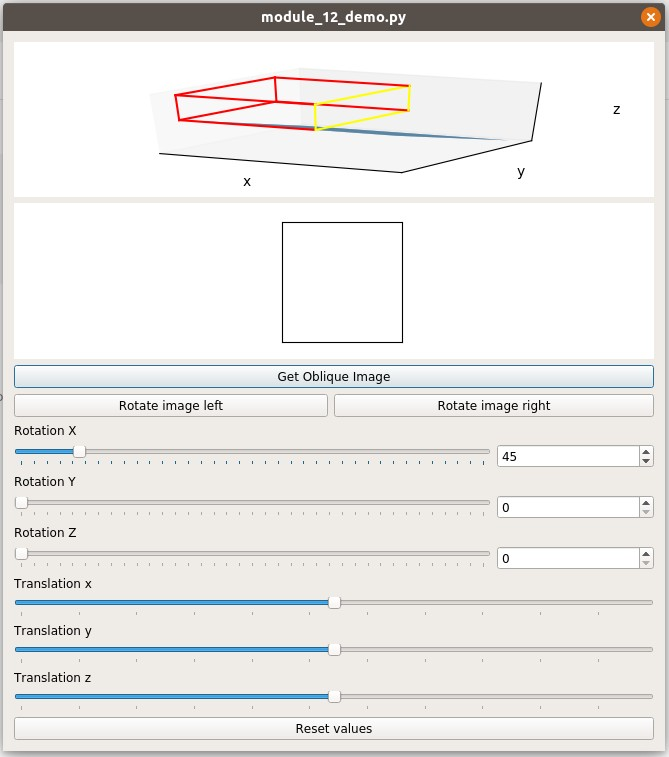
\includegraphics[scale=0.7]{figures/module_12/mod1245degrees}\caption{Grid rotated 45 degrees relative to X axis\label{fig:figure/module_12/Preprocessing}}
\end{figure}

\indent As can be seen on figure above after changing value of 'Rotation X' value in spinbox is the same as the one of the slider. Since the grid after only this rotation is under the slices and has 0 common points getting oblique image is impossible right now.
\newline\indent It is essential to translate the grid relative to Z axis. This and any other translation can be performed only by changing slider value. There are no spinboxes for that operation, because contrary to rotation, translation by any number of units doesn't mean anything if the scale is not seen

\begin{figure}[H]
\centering{}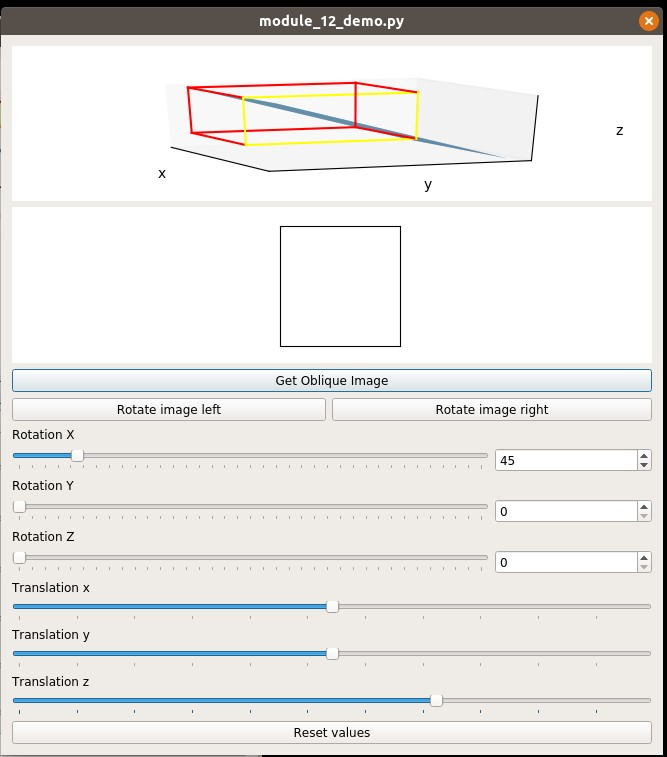
\includegraphics[scale=0.7]{figures/module_12/mod1245degreestrans}\caption{Grid rotated 45 degrees relative to X axis and translated relative to Z axis\label{fig:figure/module_12/Preprocessing}}
\end{figure}
\indent After changing the translation the grid is placed so that getting oblique image is possible. After clicking button 'Get Oblique Image' following image appears.

\begin{figure}[H]
\centering{}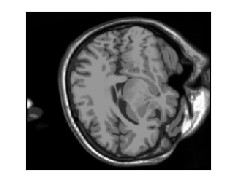
\includegraphics[scale=0.7]{figures/module_12/mod1245obl}\caption{Oblique Image obtained with parameters from previous figures\label{fig:figures/module_12/Preprocessing}}
\end{figure}

\indent For convenience of the user it is possible to rotate this image right or left by clicking 'Rotate image right' and 'Rotate image left' respectively. 

\begin{figure}[H]
\centering{}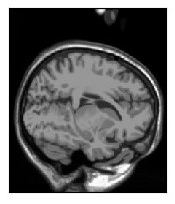
\includegraphics[scale=0.7]{figures/module_12/mod1245oblr}\caption{Oblique Image rotated right\label{fig:figures/module_12/Preprocessing}}
\end{figure}

\begin{figure}[H]
\centering{}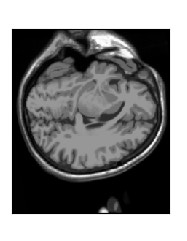
\includegraphics[scale=0.7]{figures/module_12/mod1245obll}\caption{Oblique Image rotated left\label{fig:figures/module_12/Preprocessing}}
\end{figure}

\indent Of course it is possible to rotate image infinitely number of times and every 4 times the image will be in starting orientation.
\newline\indent Clicking button 'Reset values' resets values of all sliders and spinboxes, resets upper plot to default but doesn't clear oblique image.

\begin{figure}[H]
\centering{}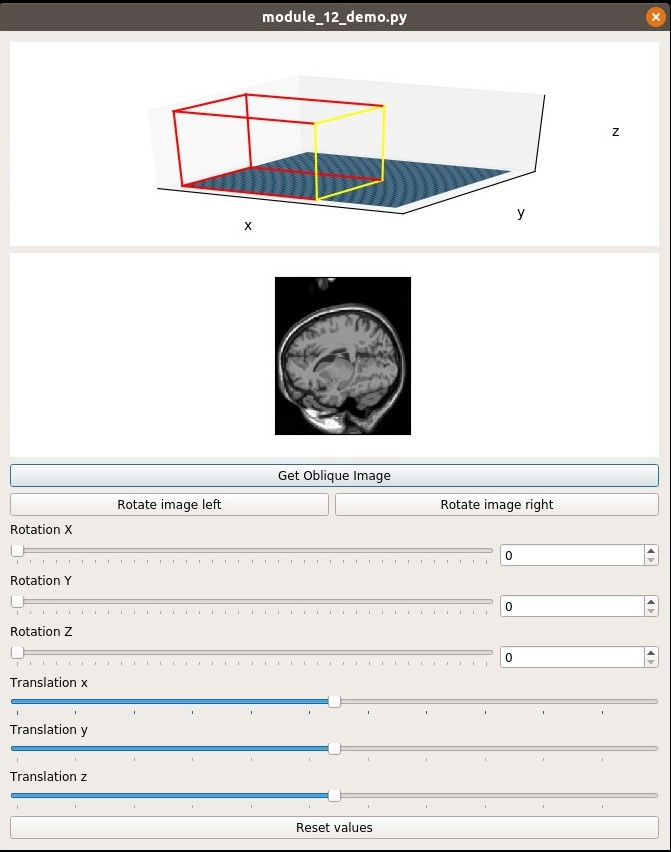
\includegraphics[scale=0.7]{figures/module_12/mod12res}\caption{Window after clicking 'Reset values' button\label{fig:figures/module_12/Preprocessing}}
\end{figure}

\textbf{Other results}
\newline\indent It is necessary to check if the module works in expected way, therefore plots and images for 3 settings are presented:
\begin{itemize}
\item Default settings
\begin{figure}[H]
\centering{}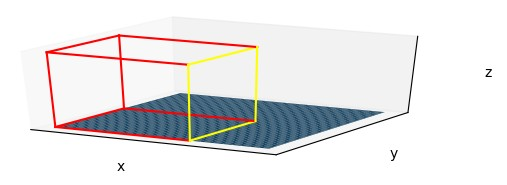
\includegraphics[scale=0.7]{figures/module_12/mod120obl}\caption{Plot with default settings\label{fig:figures/module_12/Preprocessing}}
\end{figure}


\begin{figure}[H]
\centering{}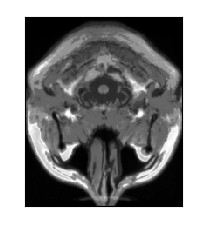
\includegraphics[scale=0.7]{figures/module_12/mod120obli}\caption{Image from default settings\label{fig:figures/module_12/Preprocessing}}
\end{figure}
\item 290 degrees rotation relative to X axis, 30 degrees rotation relative to Y axis, translated manually
\begin{figure}[H]
\centering{}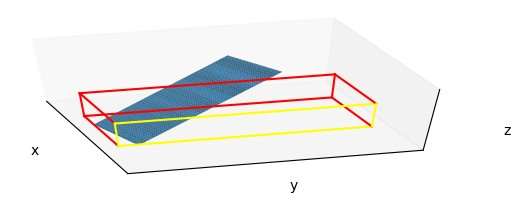
\includegraphics[scale=0.7]{figures/module_12/mod1229030}\caption{Plot with 290 degrees X, 30 degrees Y rotation and manual translation \label{fig:figures/module_12/Preprocessing}}
\end{figure}

\begin{figure}[H]
\centering{}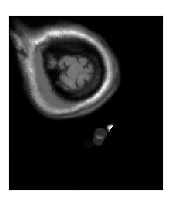
\includegraphics[scale=0.7]{figures/module_12/mod1229030obl}\caption{Image from 290 degrees X, 30 degrees Y rotation and manual translation \label{fig:figures/module_12/Preprocessing}}
\end{figure}

\item 290 degrees rotation relative to X axis, 30 degrees rotation relative to Y axis, 45 degrees relative to Z axis, translated accordingly
\begin{figure}[H]
\centering{}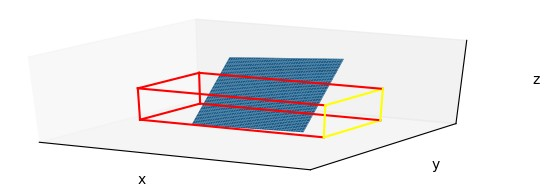
\includegraphics[scale=0.7]{figures/module_12/mod122903045}\caption{Plot with 290 degrees X, 30 degrees Y rotation, 45 degrees Z rotation and manual translation \label{fig:figures/module_12/Preprocessing}}
\end{figure}

\begin{figure}[H]
\centering{}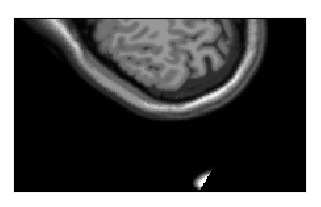
\includegraphics[scale=0.7]{figures/module_12/mod122903045obl}\caption{Image from 290 degrees X, 30 degrees Y rotation, 45 degrees Z rotation and manual translation \label{fig:figures/module_12/Preprocessing}}
\end{figure}

\end{itemize}

\indent Unfortunately it is impossible to tell if the images are interpolated correctly, because the developer does not have access to other software that performs such action. But knowing what is in places where interpolation occures if proper structures are visualized can tell if the module works properly.
\indent In order to do that the following grid was set.

\begin{figure}[H]
\centering{}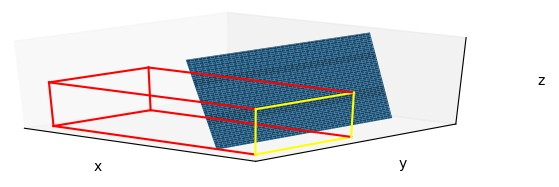
\includegraphics[scale=0.7]{figures/module_12/mod12eyes}\caption{Plot with 95 degrees X rotation and proper translation. \label{fig:figures/module_12/Preprocessing}}
\end{figure}
\indent Based on this grid an oblique image was created.
\begin{figure}[H]
\centering{}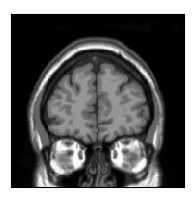
\includegraphics[scale=0.7]{figures/module_12/mod12eyesobl}\caption{Oblique image from previous settings \label{fig:figures/module_12/Preprocessing}}
\end{figure}
\indent In the picture we can see image of face, with 95 degrees X rotation at least some points were needed to be interpolated and the image looks as we could've expected. Therefore it is believed the module works just as it should.